%!TEX root = ../Thesis.tex


\section{Introduction}
This thesis will focus on \glspl{NN} which are a specific but very flexible class of \gls{ML} models that can be applied both in the supervised and unsupervised regimes as well as for \gls{RL}. This section will introduce \glspl{NN} and the three primary variations, \glspl{FNN}, \glspl{CNN} and \glspl{RNN} along with the conventional methods for training them.

\section{Fundamental types of neural networks}
\subsection{The perceptron}
Inspired by previous work on artificial neurons by McCulloch and Pitts \cite{McCulloch1943}, the first network of neurons, the perceptron, was developed by Frank Rosenblatt in 1957 \cite{Rosenblatt1957}.  Although Rosenblatt did in fact study multilayered perceptrons with some success \cite{Rosenblatt1962, Block1962}, perceptrons are often described as a single layered type of \gls{NN} \cite{Bishop2006, Goodfellow2016}. Since this view serves as a natural introduction to \glspl{NN} and in particular \glspl{FNN}, and due to the differences between the multilayered perceptrons of Rosenblatt and more modern versions, this will also be the view taken in this presentation.

Perceptrons are binary linear classifiers in that they are able to learn a linear decision boundary between two classes. Given a vector of inputs $\x\in\mathbb{R}^I$ and a vector of learnable weights $\w\in\mathbb{R}^I$ along with a scalar bias parameter $b\in\mathbb{R}$, the perceptron computes a binary response $y\in\cbra{-1,1}$ by the following linear transformation.
\begin{equation}
    y = \varphi\pa{\sum_{i=1}^I w_ix_i + b_i} = \varphi\pa{\w\transpose\x + b}
\end{equation}
where 
\begin{equation}
    \varphi(z) = \begin{cases}
                    1 & \text{if } z\geq0\\
                    -1 & \text{if } z<0
                 \end{cases}
\end{equation}
is a binarizing, or step, \textit{activation function}. More compactly, the bias parameter can be included by introducing an artificial, or dummy, feature in $\x$ with the constant value of $1$ and defining the bias to be the associated new element in $\w$. Then  
\begin{equation}\label{eq: Machine learning: Perceptron forward no bias}
    y = \varphi\pa{\sum_{i=1}^{I+1} w_ix_i} = \varphi\pa{\w\transpose\x}
\end{equation}
where now $\x, \w\in\mathbb{R}^{I+1}$ \cite{Bishop2006}.

Perceptrons, as well as all other \gls{NN} models, can be represented as a computational graph. Such a representation of the perceptron without explicit biases can be seen in \autoref{fig: Neural networks: Perceptron}. Each node of the graph represents a single real number and every edge leaving some input layer node represents the multiplication of that input with a specific learnable weight. The incidence of the $I$ edges on the output node represents the summation of these products to form a weighted sum of the inputs. As per the definition above, the output is then computed by application of the activation function $\varphi$ to the weighted sum of inputs.
\begin{figure}[tbp!]
    \begin{subfigure}[b]{0.40\textwidth}
        \centering
        \begin{tikzpicture}[x=1.0cm, y=1.0cm, >=stealth, font=\sffamily\scriptsize]
    \tikzstyle{every neuron}=[circle, draw, minimum size=.6cm]
    \tikzstyle{neuron missing}=[draw=none, scale=2, text height=0.333cm, execute at begin node={\color{black}\tiny$\vdots$}]
    
    % Input nodes
    \foreach \m/\l [count=\y] in {1,2,3,missing,4}
        \node [every neuron/.try, neuron \m/.try] (input-\m) at (0,2.5-\y) {};
      
    % Output node
    \node [every neuron/.try, neuron 1/.try ] (output-1) at (2,1.5-1) {};

    % Names on input arrows
    \foreach \l [count=\i] in {1,2,3,I}
        \draw [<-] (input-\i) -- ++(-1,0) node [above, midway] {$x_\l$};
    
    % Name on output arrow
    \draw [->] (output-1) -- ++(1,0) node [above, midway] {$y$};
    
    % Inputs -> Outputs
    \draw [->] (input-1) -- node[above right]{$w_{1}$} (output-1);
    \draw [->] (input-2) -- (output-1);
    \draw [->] (input-3) -- (output-1);
    \draw [->] (input-4) -- node[below right]{$w_{I}$} (output-1);
    
    % Layer names
    \foreach \l [count=\x from 0] in {Input\\layer, Output\\layer}
        \node [align=center, above] at (\x*2,2) {\l};
\end{tikzpicture}
        \caption{}
        \label{fig: Neural networks: Perceptron}
    \end{subfigure}
    \hfill
    \begin{subfigure}[b]{0.58\textwidth}
        \centering
        \begin{tikzpicture}[x=1.0cm, y=1.0cm, >=stealth, font=\sffamily\scriptsize]
    \tikzstyle{every neuron}=[circle, draw, minimum size=.6cm]
    \tikzstyle{neuron missing}=[draw=none, scale=2, text height=0.333cm, execute at begin node={\color{black}\tiny$\vdots$}]
    
    % Inputs nodes
    \foreach \m/\l [count=\y] in {1,2,3,missing,4}
      \node [every neuron/.try, neuron \m/.try] (input-\m) at (0,2.5-\y) {};
      
    % Hidden nodes
    \foreach \m [count=\y] in {1,missing,2} {
        \node [every neuron/.try, neuron \m/.try ] (hidden-\m) at (2,2-\y*1.25) {};
    }
        % \ifthenelse{\y=2}
        %     {\node [every neuron/.try, neuron \m/.try ] (hidden-\m) at (2,2-\y*1.25) {};}
        %     {\node [every neuron/.try, neuron \m/.try ] (hidden-\m) at (2,2-\y*1.25) {$a_\m^\bra{0}$};}
        % }
      %\node [every neuron/.try, neuron \m/.try ] (hidden-\m) at (2,2-\y*1.25) {$a_\m^\bra{0}$};
      
    % Outputs nodes
    \foreach \m [count=\y] in {1,missing,2}
      \node [every neuron/.try, neuron \m/.try ] (output-\m) at (4,1.5-\y) {};
      
    % Names on inputs
    \foreach \l [count=\i] in {1,2,3,I}
      \draw [<-] (input-\i) -- ++(-1,0)
        node [above, midway] {$x_\l$};
        
    % Names on hidden
    \foreach \l [count=\i] in {1,H} {
        \ifthenelse{\i=1}
            {\node [above] at (hidden-\i.north) {$z^\bra{1}_\l$};}
            {\node [below] at (hidden-\i.south) {$z^\bra{1}_\l$};}
    }
      
    % Names on outputs
    \foreach \l [count=\i] in {1,O}
      \draw [->] (output-\i) -- ++(1,0)
        node [above, midway] {$y_\l$};
        
    % Inputs -> Hidden
    \foreach \i in {1,...,4} {
      \foreach \j in {1,...,2} {
        %\draw [->] (input-\i) -- (hidden-\j);
        \ifthenelse{\i=1 \AND \j=1 \OR \i=4 \AND \j=2}
            {}
            {\draw [->] (input-\i) -- (hidden-\j);}
        }
    }
    \draw [->] (input-1) --node[above]{$W^{\bra{1}}_{1,1}$} (hidden-1);
    \draw [->] (input-4) --node[below]{$W^{\bra{1}}_{H,I}$} (hidden-2);
        
    % Hidden -> Outputs
    \foreach \i in {1,...,2}  {
      \foreach \j in {1,...,2} {
        % \draw [->] (hidden-\i) -- (output-\j);
        \ifthenelse{\i=1 \AND \j=1 \OR \i=2 \AND \j=2}
            {}
            {\draw [->] (hidden-\i) -- (output-\j);}
        }
    }
    \draw [->] (hidden-1) --node[above]{$W^{\bra{2}}_{1,1}$} (output-1);
    \draw [->] (hidden-2) --node[below]{$W^{\bra{2}}_{O,H}$} (output-2);
    
    % Layer names
    \foreach \l [count=\x from 0] in {Input, Hidden, Output}
      \node [align=center, above] at (\x*2,2) {\l \\ layer};
\end{tikzpicture}
        \caption{}
        \label{fig: Neural networks: MLP}
    \end{subfigure}
    \caption{\subref{fig: Neural networks: Perceptron} A scalar computational graph of the perceptron model due to Rosenblatt \cite{Rosenblatt1957}. The single scalar output is computed as the sign of the weighted sum of inputs. This is similar to the McCulloch-Pitts neuron \cite{McCulloch1943}. \subref{fig: Neural networks: MLP} A scalar computational graph for a modern two-layer \gls{FNN} with a single hidden layer and an output layer, $L=2$. The output vector is computed through a series of affine transformations and associated nonlinear activation functions.}
    \label{fig: Neural networks: Single and multilayer perceptron (FNN)}
\end{figure}

A straightforward way to define a learning algorithm for a perceptron is through error function minimization\footnote{Within \gls{ML}, \textit{error function} is the widely used term for what is generally called the \textit{objective function} in optimization. The name \textit{cost function} is also often used while the term \textit{loss function} can be used to mean the same but sometimes also refers to the error or cost associated with a single training example.}. In error function minimization, a measure of the amount of error made by a model on a training set is defined and evaluated. Some optimization algorithm can then be applied to the gradient, and potentially the Hessian, of the error function in order to update the model parameters in the direction of decreasing error. 
An error function useful for training perceptrons is the so-called \textit{perceptron criteria} given by
\begin{equation}
    E_\text{P}(\w) = -\frac{1}{N}\sum_{n\in\mathcal{M}}\w\transpose\x_n t_n
\end{equation}
where $t_n$ is the $n$'th target in a training set of $N$ examples, and $\mathcal{M}=\cbra{n \mid y_n\ne t_n}$ is the set of misclassifications. Since $t_n>0$ requires $\w\transpose\x_n<0$ for $n$ to be misclassified, and vice versa, this error function measures the total amount of error made in misclassified samples and has a minimum of zero when $\mathcal{M}$ is empty. 
It can be noted that since $E_\text{P}$ is zero in any region of $\w$ space that makes correct classifications and depends linearly on $\w$ in regions resulting in incorrect classifications, it is a piecewise linear function.
The gradient of this error function w.r.t. the weights is
\begin{equation}
    \nabla_\w E_\text{P}(\w) = -\frac{1}{N}\sum_{n\in\mathcal{M}}\x_n t_n
\end{equation}
and the Hessian is clearly zero. The gradient can be directly used for regular gradient descent or \gls{SGD} which uses a single training example to evaluate the gradient at each iteration, saving computation but also introducing stochasticity. The gradient descent update is
\begin{equation}
    \w \leftarrow \w -\eta\nabla_\w E_\text{P}(\w) = \w+\frac{1}{\size{\mathcal{B}}}\sum_{n\in\mathcal{B}}\x_n t_n \ ,
\end{equation}
where the batch $\mathcal{B}$ is equal to $\mathcal{M}$ for regular gradient descent. Whenever $\size{\mathcal{M}}>\size{\mathcal{B}}>1$ the gradient descent scheme above is called mini-batch \gls{SGD}. In the above, $\eta$ has been set to one without loss of generality since multiplication of $\w$ by any positive constant does not change the perceptron output $y$ \cite{Bishop2006}.


\subsection{Feedforward neural networks}
\glsreset{FNN}
\Glspl{FNN} are conceptually a simple extension of perceptrons that contain multiple perceptron units in a layered feedforward fashion. Therefore, they are also known as \glspl{MLP}.

An \gls{FNN} can be represented mathematically by a series of affine transformations followed by a nonlinear activation function. Let $\a^{\bra{0}}=\x$. The transformation applied between layers $l$ and $l+1$ when forward propagating the input $\x$ can then be written as
\begin{equation}\label{eq: Neural networks: Feedforward neural network forward pass for l'th layer}
    \begin{aligned}
        \z^{\bra{l+1}} &= \W^{\bra{l+1}}\a^{\bra{l}} + \b^{\bra{l+1}}\\
        \a^{\bra{l+1}} &= \varphi_{l+1}\pa{\z^{\bra{l+1}}}
    \end{aligned}
     \ ,  \quad l\in[0,L-1]
\end{equation}
where $\varphi_l$ is the activation function, or non-linearity, of the $l$'th layer, square brackets denote layer indexing and $L$ is the total number of layers in the network. The $\z$ variables are often called \textit{hidden units} while $\a$ are called \textit{hidden unit activations}, or simply \textit{activations}. Often, the \gls{NN} output activations are denoted by $\y$ such that $\y=\a^{\bra{L}}$ and the last layer activation is often different from the internal ones depending on application. The computation of an \gls{NN} output from an input is called the \textit{forward pass} or \textit{forward propagation} \cite{Goodfellow2016}. \autoref{fig: Neural networks: MLP} shows the computational graph of a general two-layer \gls{FNN} without explicit biases. 

The first layer matrix is restricted to have $I$ columns due to the input dimension. The remaining dimensions of all weight matrices then define the size of the \gls{FNN} with biases $\b^{\bra{l}}$ always being vectors of the same dimensionality as the rows in the corresponding weight matrix, $\W^{\bra{l}}$.

To further illustrate the connection to perceptrons, note that the first row of the $\W^{\bra{l}}$ matrix holds the weights of the perceptron model that describes the connection between $\z^{\bra{l}}$ and $z^{\bra{l+1}}_1$. For example, the $a_1$ activation is computed as follows.
\begin{equation}
    \begin{aligned}
        z_1^\bra{1} &= \sum_{i=1}^I W_{1,i}^{\bra{1}} x_i = \W_{1,:}^{\bra{1}}\transpose\x\\
        a_1^\bra{1} &= \varphi\pa{z_1^\bra{1}}
    \end{aligned}
\end{equation}
which is equivalent to the equation of a single perceptron defined in \eqref{eq: Machine learning: Perceptron forward no bias}. As such, each layer of an \gls{FNN} consists of a number of perceptron models. Following layers then use the outputs of preceeding perceptrons as input.

Besides the multilayered structure, one major difference between \glspl{FNN} and perceptrons is the use of real-valued activation functions. Where the perceptron used a binary threshold based activation function, modern \glspl{FNN} typically use nonlinear, real-valued activation functions which are applied elementwise to the hidden units to form the activations. Development of new activation functions is an active field of research. Classical activation functions were the sigmoid $\sigma(\cdot)$ and the hyperbolic tangent,
\begin{align}
    \sigma(\z) &= \frac{1}{1+\exp(-\z)} = \frac{\exp(\z)}{1+\exp(\z)}\\
    \tanh(\z) &= \frac{\exp(\z)-\exp(-\z)}{\exp(\z)-\exp(-\z)} = 2\sigma(2\z) - 1 \ .
\end{align}
These functions are constrained to values in $\bra{0, 1}$ and $\bra{-1,1}$, respectively, but suffer from extremely small gradients for inputs with large absolute values. Due to the way modern \glspl{NN} are trained, this often risks slowing down or completely stopping training. More modern activation functions include the \gls{ReLU} \cite{Glorot2011} and the softplus,
\begin{align}
    \text{ReLU}(\z) &= \max\cbra{0,\z}\\
    \text{softplus}(\z) &= \log\pa{1+\exp(\z)} \ ,
\end{align}
as well as many others. These generally seek to avoid small gradients while still being nonlinear, easy to compute and retaining some nice properties such as monotonicity.
The chosen activations need not generally be the same throughout the network. In fact, the activation applied to the output layer is most often not and instead depends on the application. For regression tasks, the output layer often omits the activation function altogether since outputs are many times unbounded. For binary classification tasks, the sigmoid activation can be applied to an output layer with $1$ unit, resulting in a logistic regression model. For multiclass classification with $K$ classes, the softmax,
\begin{equation}
    \text{softmax}(\z) = \frac{\exp\pa{\z}}{\sum_{i=1}^K \exp\pa{z_i}} \ ,
\end{equation}
is commonly applied to an output layer with $K$ units \cite{Goodfellow2016}.

%Compared with these deep \glspl{FNN}, perceptrons seem almost naively simplistic considering the fairly straightforward mathematical generalization required to obtain multilayered networks. However, early perceptrons were in fact implemented in circuitry which made multilayered structures difficult to create \cite{Rosenblatt1957}. Additionally, the training algorithm used for perceptrons did not easily generalize to multiple layers and non-binary responses .


\subsection{Convolutional neural networks}
A \Gls{CNN} is a type of \gls{NN} that uses the convolution operation rather than the affine transformation employed by \glspl{FNN}. The \gls{CNN} was first introduced in the form of the Neocognitron in 1980 \cite{Fukushima1980}. After the popularization of backpropagation, a network with one-dimensional convolutions was first trained with this algorithm in 1988 \cite{Hinton1988} and with two-dimensional convolutions for handwritten digit recognition in 1989 \cite{LeCun1989a}. The superior performance of \glspl{CNN} on image classification tasks compared to alternative methods was demonstrated in a 1998 paper by LeCun et al. \cite{LeCun1998}.

The discrete one-dimensional convolution is written as $\s = \x*\k$ for an input vector $\x$ and a \textit{convolution kernel} $\k$. Each element of the output \textit{feature map} $\s$ is computed as
\begin{equation}\label{eq: Neural network: 1D convolution}
    s_{i} = \sum_n x_{i+n} k_n \ .
\end{equation}
with $n$ iterating all indices in $\k$. The dimension of $\s$ does not equal the dimension of $\x$.
The two-dimensional convolution can be written as $\S = \X*\K$ with
\begin{equation}\label{eq: Neural network: 2D convolution}
    S_{i,j} = \sum_n\sum_m X_{i+n,j+m}K_{m,n}
\end{equation}
and matrix input, kernel and feature map\footnote{In fact, this operation is called \textit{cross-correlation} while the one- and two-dimensional discrete convolutions are defined as
\begin{align*}
    s_{i} &= \sum_n x_{i-n} k_n\\
    S_{i,j} &= \sum_n\sum_m X_{i-n,j-m}K_{m,n} \ .
\end{align*}
These correspond to flipping each dimension of the kernel used in the above definition and makes the operation commutative. In practice, the kernel parameters of a \gls{CNN} are learned and the commutative property is not used. Thus, the two operations are equally applicable and result in the same performance. In machine learning, the cross-correlation is often simply called convolution and used in its place. As will be done here.} \cite{Goodfellow2016}. The two-dimensional convolution is illustrated graphically in \autoref{fig: Neural networks: no_padding_no_strides}. 
\begin{figure}[tbp!]
    \begin{subfigure}[b]{0.24\textwidth}
        \centering
        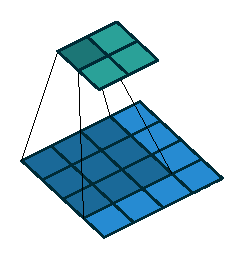
\includegraphics[width=\textwidth]{graphics/neuralnetworks/no_padding_no_strides_00.pdf}
        \caption{}
        \label{fig: Neural networks: no_padding_no_strides_00}
    \end{subfigure}
    \hfill
    \begin{subfigure}[b]{0.24\textwidth}
        \centering
        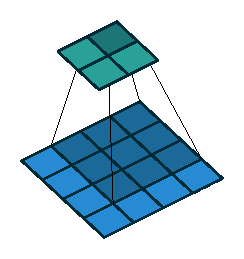
\includegraphics[width=\textwidth]{graphics/neuralnetworks/no_padding_no_strides_01.pdf}
        \caption{}
        \label{fig: Neural networks: no_padding_no_strides_01}
    \end{subfigure}
    \hfill
    \begin{subfigure}[b]{0.24\textwidth}
        \centering
        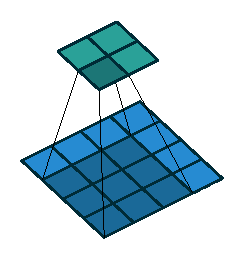
\includegraphics[width=\textwidth]{graphics/neuralnetworks/no_padding_no_strides_02.pdf}
        \caption{}
        \label{fig: Neural networks: no_padding_no_strides_02}
    \end{subfigure}
    \hfill
    \begin{subfigure}[b]{0.24\textwidth}
        \centering
        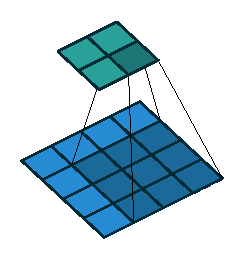
\includegraphics[width=\textwidth]{graphics/neuralnetworks/no_padding_no_strides_03.pdf}
        \caption{}
        \label{fig: Neural networks: no_padding_no_strides_03}
    \end{subfigure}
    \caption{Convolution of a $(4\times4)$ input with a $(3\times3)$ kernel to form a $(2\times2)$ output in four steps. Similarly to the affine transformation of \glspl{FNN}, each output element is a weighted sum of the inputs. The weights are learnable and conversely to \glspl{FNN} they are shared across the input. See also \autoref{fig: Neural networks: numerical_no_padding_no_strides}. Figures due to \cite{Dumoulin2018}.}
    \label{fig: Neural networks: no_padding_no_strides}
\end{figure}

The convolution operation can be formulated as a matrix-vector multiplication. This is demonstrated here by convolution of a $3\times3$ input by a $2\times2$ kernel to form a $2\times2$ feature map. The input is unrolled into columns of the elements acted on by the kernel at each position. The input then forms a symmetric matrix. This is multiplied by the kernel unrolled to a column vector. This can be written as,
\begin{align*}
    \S
    &= \X * \K\\
    &=  \bmat{
            X_{11} & X_{21} & X_{31}\\
            X_{12} & X_{22} & X_{32}\\
            X_{13} & X_{23} & X_{33}
        } * 
        \bmat{
            K_{11} & K_{12}\\
            K_{21} & K_{22}
        }\\
    &=  \bmat{
            X_{11} & X_{12} & X_{21} & X_{22}\\
            X_{12} & X_{13} & X_{22} & X_{23}\\
            X_{21} & X_{22} & X_{31} & X_{32}\\
            X_{22} & X_{23} & X_{32} & X_{33}\\
        }
        \bmat{
            K_{11} \\ K_{12} \\ K_{21} \\ K_{22}
        }_{2\times2}\\
    &=  \bmat{
            K_{11}X_{11} + K_{12}X_{12} + K_{21}X_{21} + K_{22}X_{22}\\
            K_{11}X_{12} + K_{12}X_{13} + K_{21}X_{22} + K_{22}X_{23}\\
            K_{11}X_{21} + K_{12}X_{22} + K_{21}X_{31} + K_{22}X_{32}\\
            K_{11}X_{22} + K_{12}X_{23} + K_{21}X_{32} + K_{22}X_{33}
        }_{2\times2} \ . %\\
    % &=  \bmat{
    %         K_{11}X_{11} + K_{12}X_{12} + K_{21}X_{21} + K_{22}X_{22} &
    %         K_{11}X_{12} + K_{12}X_{13} + K_{21}X_{22} + K_{22}X_{23}\\
    %         K_{11}X_{21} + K_{12}X_{22} + K_{21}X_{31} + K_{22}X_{32} &
    %         K_{11}X_{22} + K_{12}X_{23} + K_{21}X_{32} + K_{22}X_{33}
%        }.
\end{align*}
Note how each feature map element is computed as a weighted sum of the corresponding input elements with the weights defined by the kernel. This is visualized in \autoref{fig: Neural networks: numerical_no_padding_no_strides}. This matrix-vector formulation easily extends to multiple kernels resulting in multiple feature maps by adding additional kernels as columns to the unrolled kernel. Efficient algorithms for computing the convolution is still an active research field \cite{Goodfellow2016}
\begin{figure}[tbp!]
    \begin{subfigure}[b]{0.49\textwidth}
        \centering
        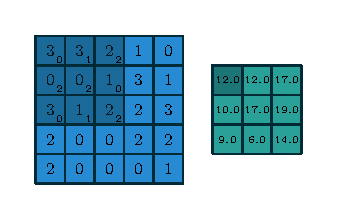
\includegraphics[width=\textwidth]{graphics/neuralnetworks/numerical_no_padding_no_strides_00.pdf}
        \caption{}
        \label{fig: Neural networks: numerical_no_padding_no_strides 1}
    \end{subfigure}
    \hfill
    \begin{subfigure}[b]{0.49\textwidth}
        \centering
        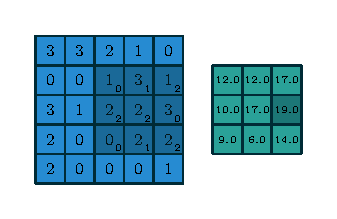
\includegraphics[width=\textwidth]{graphics/neuralnetworks/numerical_no_padding_no_strides_05.pdf}
        \caption{}
        \label{fig: Neural networks: numerical_no_padding_no_strides 2}
    \end{subfigure}
    \caption{Convolution of a $(5\times5)$ input with a $(3\times3)$ kernel to form a $(3\times3)$ output exemplified by two out of a total of nine required steps. It is shown how each feature map element is a weighted sum of the input with the kernel as weights. Figures due to \cite{Dumoulin2018}.}
    \label{fig: Neural networks: numerical_no_padding_no_strides}
\end{figure}

The convolution operation leverages three ideas that separate it from the affine transformation \cite{Goodfellow2016}.
\begin{enumerate}
    \item Sparse connectivity
    \item Parameter sharing
    \item Equivariant representations
\end{enumerate}
These are introduced briefly below.

The \textit{sparse connectivity} arises from each kernel being smaller than the input. Each unit of the feature map is then a function of only part of the input proportional to the kernel size. This also gives rise to the concept of the \textit{local receptive field} which is defined as the range of inputs which are connected to a certain feature map element. The layer that is connected to the input has a receptive field defined by its own kernel size. By stacking convolutional layers, the receptive field increases in size by indirectly connecting to a wider range of inputs through the feature maps of preceeding layers \cite{Goodfellow2016}.

\textit{Parameter sharing} is introduced by letting the kernel act on the entire input image by sliding it across it. Each element in the feature map then depends on learning a kernel that is useful for many locations in the input, This allows a \gls{CNN} to exploit correlations between neighbouring elements in the input. In the case of time series or images this corresponds to exploiting temporal or spatial correlations, irrespective of their specific locations within the input. This is not possible for an \gls{FNN} \cite{Goodfellow2016}. 

The convolution is \textit{equivariant to translations} in its input in the sense that for any translation operation $T$ applied to $\X$ it holds that
\begin{equation}
    T\bra{\X} * \K = T\bra{\X * \K} = \X * T\bra{\K}
\end{equation}
i.e. applying the translation to the input (or kernel) and doing the convolution is equivalent to doing the convolution and then applying the translation to the feature map\footnote{Equivariance differs from invariance. Where equivariance means that output changes in the same way as input does, invariance to a transformation means that output does not change when that transformation is applied to the input. Often, invariance can be obtained fairly easily from equivariance by disregarding the additional information about the input transformation contained in the output \cite{Goodfellow2016}. There has been some discussion of these properties in relation to the newly proposed capsule networks \cite{Sabour2017} as an alternative to \glspl{CNN}.} \cite{Goodfellow2016}.

Beside the input size and kernel size, some other parameters that define the convolution operation are input zero \textit{padding}, the distance between two consecutive positions of the kernel on the input called the \textit{stride}, and \textit{dilation} which controls the distance between the inputs read by the kernel at a single position \cite{Dumoulin2018}.

\begin{figure}[tbp!]
    \begin{subfigure}[b]{0.49\textwidth}
        \centering
        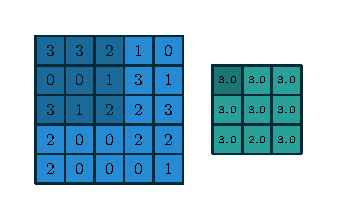
\includegraphics[width=\textwidth]{graphics/neuralnetworks/numerical_max_pooling_00.pdf}
        \caption{}
        \label{fig: Neural networks: numnumerical_max_pooling_00}
    \end{subfigure}
    \hfill
    \begin{subfigure}[b]{0.49\textwidth}
        \centering
        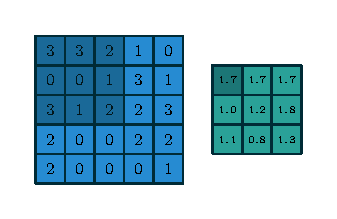
\includegraphics[width=\textwidth]{graphics/neuralnetworks/numerical_average_pooling_00.pdf}
        \caption{}
        \label{fig: Neural networks: numerical_average_pooling_00}
    \end{subfigure}
    \caption{\subref{fig: Neural networks: numnumerical_max_pooling_00} Max- and \subref{fig: Neural networks: numerical_average_pooling_00} average-pooling of a $(5\times5)$ input with a $(3\times3)$ kernel to form a $(3\times3)$. Figures due to \cite{Dumoulin2018}.}
    \label{fig: Neural networks: numerical_pooling}
\end{figure}
In order to shrink the dimension of resulting feature maps, pooling layers are often applied after convolutional layers. Generally, pooling layers summarize a neighbourhood of elements in a feature map into a single element by using some operation. The most widespread type of pooling is max-pooling \cite{Zhou1988, Ranzato2007, Scherer2010}. 
% Here the individual
% \begin{equation}
%     \tilde{S}_{i,j} = \max\cbra{S_{n,m}\mid m\in\bra{i-\frac{n-1}{2},i+\frac{n-1}{2}}, m\in\bra{j-\frac{m-1}{2},j+\frac{m-1}{2}}}
% \end{equation}
When max-pooling is applied to a two dimensional input, each element of the resulting feature map is computed as the maximum element contained within a rectangular pooling kernel applied to the input, similarly to how convolution is computed, by sliding the kernel. Other types of pooling apply a different operation, e.g. averaging, weighted averaging according to distance from center and $L_2$ norm \cite{Goodfellow2016}. Max- and average-pooling are illustrated in \autoref{fig: Neural networks: numerical_pooling}. These pooling operations can make convolution \textit{invariant to translations}, such that output does not change for small translations of the input. When learning multiple kernels in a single convolutional layer and pooling over these, additional invariances, such as rotation invariance, can be learned \cite{Goodfellow2016}.

Conventionally, \glspl{CNN} consist of a series of convolutional layers each followed by a pooling layer and an activation function with the final convolutional layer feature map being flattened and input to an \gls{FNN}, e.g. for classification. In \cite{Lin2013} it was proposed to dispense with the fully connected layers by having the final convolutional layer output a feature map for each of the $K$ classes and averaging them to form a $K$ dimensional vector which is then fed to the softmax activation. Another attempt at making \glspl{CNN} fully convolutional was made in \cite{Long2015}.


\subsection{Recurrent neural networks}
\begin{figure}[tbp!]
    \begin{subfigure}[b]{0.25\textwidth}
        \centering
        \resizebox{!}{3cm}{
            \begin{tikzpicture}[x=1cm, y=1cm, >=stealth, font=\sffamily\scriptsize]
    \tikzstyle{neuron}=[circle, draw, minimum size=.6cm]
    \tikzstyle{Arrow}=[rounded corners=.20cm,thick] % Arrows with rounded corners
    \tikzstyle{cell}=[% For the main box
        rectangle,
        draw,
        rounded corners=1mm,
        very thick,
        minimum width=6mm,
        minimum height=4mm,
        inner sep=3pt
        ]
    % Input node
    \node [neuron] (input) at (0,0) {$\x^\vbra{t}$};
    
    % Recurrent cell
    \node [cell] (cell) at (0,1) {RNN cell};
    
    % Output node
    \node [neuron] (output) at (0,2) {$\h^\vbra{t}$};
    
    % Feedforward arrows
    \draw [->, Arrow] (input) -- (cell);
    \draw [->, Arrow] (cell) -- (output);
    
    % Feedback arrows
    \draw [-, Arrow] (cell.east) -- (1, 1) -- (1, 1.325) -- (0.2, 1.325);
    \draw [<-, Arrow] (cell.west) -- (-1, 1) -- (-1, 1.325) -- (-0.2, 1.325);
\end{tikzpicture}
        }
        \caption{}
        \label{fig: Neural networks: RNN}
    \end{subfigure}
    \hfill
    \begin{subfigure}[b]{0.73\textwidth}
        \centering
        \resizebox{!}{3cm}{
            \newcommand{\empt}[2]{$#1^{\langle #2 \rangle}$}
\begin{tikzpicture}[x=1cm, y=1cm, >=stealth, font=\sffamily\scriptsize]
    \tikzstyle{neuron}=[circle, draw, minimum size=.6cm]
    \tikzstyle{dots}=[draw=none, scale=2, text height=0.333cm, execute at begin node={\color{black}\tiny$\cdots$}]
    \tikzstyle{Arrow}=[rounded corners=.20cm,thick] % Arrows with rounded corners
    \tikzstyle{cell}=[% For the main box
        rectangle,
        draw,
        rounded corners=1mm,
        very thick,
        minimum width=6mm,
        minimum height=4mm,
        inner sep=3pt
        ]
    
    % Input nodes
    \node [neuron] (input1) at (0,0) {\empt{\x}{1}};
    \node [neuron] (input2) at (2,0) {\empt{\x}{2}};
    \node [neuron] (inputT) at (6,0) {\empt{\x}{T}};
    
    % Recurrent cells
    \node [cell] (cell1) at (0,1) {RNN cell};
    \node [cell] (cell2) at (2,1) {RNN cell};
    \node [cell] (cellT) at (6,1) {RNN cell};
    
    % Hidden nodes
    \node [neuron] (hidden0) at (-1.5,1) {\empt{\h}{0}};
    \node [neuron] (hidden1) at (0,2) {\empt{\h}{1}};
    \node [neuron] (hidden2) at (2,2) {\empt{\h}{2}};
    \node [neuron] (hiddenT) at (6,2) {\empt{\h}{T}};
    
    % Dots
    \node [neuron, draw=none, scale=2] (dots1) at (4,1) {\tiny$\dots$};
    
    % Hidden to cell to cell ... to cell
    \draw [->, Arrow] (hidden0) -- (cell1);
    \draw [->, Arrow] (cell1) -- (cell2);
    \draw [->, Arrow] (cell2) -- (dots1);
    \draw [->, Arrow] (dots1) -- (cellT);
    
    % Input to cell to hidden
    \draw [->, Arrow] (input1) -> (cell1) -- (hidden1);
    \draw [->, Arrow] (input2) -> (cell2) -- (hidden2);
    \draw [->, Arrow] (inputT) -> (cellT) -- (hiddenT);
\end{tikzpicture}
        }
        \caption{}
        \label{fig: Neural networks: RNN unrolled}
    \end{subfigure}
    \caption{\subref{fig: Neural networks: RNN} Illustration of the feedback loop in a basic \gls{RNN}. Without the feedback this would have been an ordinary \gls{FNN}. \subref{fig: Neural networks: RNN unrolled} The same \gls{RNN} but unrolled in time. Each recurrent cell applies the same set of operations recurrently on each input element and updated hidden state. Figures inspired by \cite{Olah2015}.}
    \label{fig: Neural networks: RNNs}
\end{figure}
\Glspl{RNN} \cite{Rumelhart1986} are a type of neural networks specialized for processing sequential data of variable length. 
Given an input sequence $\cbra{\x^\vbra{t}}_{t=1}^{T}=\cbra{\x^\vbra{1}, \x^\vbra{2}, \dots, \x^\vbra{T}}$ of length $T$ an \gls{RNN} recurrently applies the same series of operations to each sequence time step, $\x^\vbra{t}$, starting from one end or both ends if the \gls{RNN} is \textit{bidirectional}. The power of \glspl{RNN} lie in the ability to compute some hidden state which changes depending on the entire history of seen sequence vectors. This works as a kind of memory.

An \gls{RNN} can be represented as a computational graph with a feedback loop as in \autoref{fig: Neural networks: RNN}. There, the entire sequence $\x$ is the input and the RNN cell outputs the hidden state $\h$. Such a graph can be unrolled to the length of the input sequence as seen in \autoref{fig: Neural networks: RNN unrolled}. It is then clear how the input sequence is read element by element while the hidden state is updated. The hidden state sequence may have a length different from the length of the input sequence. A length of $1$ for the hidden state sequence is typically used for classification. There is no requirement that a hidden state must be output whenever a input is read. In fact, an \gls{RNN} can consist of an encoder which first reads the input sequence and a decoder which then constructs the output.
\begin{figure}[tbp!]
    \centering
    \newcommand{\empt}[2]{$#1^{\langle #2 \rangle}$}
\begin{tikzpicture}[
    % GLOBAL CFG
    font=\sffamily\scriptsize,
    >=LaTeX,
    % Styles
    cell/.style={% For the main box
        rectangle, 
        rounded corners=5mm, 
        draw,
        very thick,
        },
    vector/.style={% For external inputs and outputs
        circle,
        draw,
        line width = .75pt,
        minimum width=1cm,
        inner sep=1pt,
        },
    gate/.style={% For internal inputs
        rectangle,
        draw,
        minimum width=4mm,
        minimum height=3mm,
        inner sep=1pt
        },
    mylabel/.style={% something new that I have learned
        font=\scriptsize\sffamily
        },
    ArrowC1/.style={% Arrows with rounded corners
        rounded corners=.25cm,
        thick,
        }
    ]

    % Cell
    \node [cell, minimum height=4cm, minimum width=6cm] at (0,0){} ;
    
    % Inputs
    \node[vector, label={[mylabel]Hidden}] (h) at (-4,1.5) {\empt{\h}{t-1}};
    \node[vector, label={[mylabel]left:Input}] (x) at (-2.5,-3) {\empt{\x}{t}};
    
    % Outputs
    \node[vector, label={[mylabel]Hidden}] (h2) at (4,1.5) {\empt{\h}{t}};
    \node[vector, label={[mylabel]left:Hidden}] (h22) at (2.5,3) {\empt{\h}{t}};
    
    \node [gate, minimum width=1cm] (hiddengate) at (0,0) {tanh};

    % Coordinates
    \coordinate(hiddenbend) at (-2,1.5);
    \coordinate(inputbend) at (-2.5,-1);
    \coordinate(hxjoin) at (-2,-1);
    \coordinate(bendbelowtanh) at (0,-1);
    \coordinate(bendabovetanh) at (0,1.5);
    \coordinate(hiddensplit) at (2.5,1.5);

    % Arrows
    \draw [ArrowC1] (h) -- (hiddenbend) -- (hxjoin) -- (bendbelowtanh) -- (hiddengate);
    \draw [ArrowC1] (x) -- (inputbend) -- (hxjoin)--++(0.5,0);
    \draw [ArrowC1] (hiddengate) -- (bendabovetanh) -- (h2);
    \draw [ArrowC1] (hiddensplit)++(-0.5,0) -- (hiddensplit) -- (h22);
\end{tikzpicture}
    \caption{Layout of the basic recurrent cell. Due to the small gradients of the $\tanh$, this cell is often not able to propagate error signals far enough back in time to learn long term dependencies. Figure inspired by \cite{Olah2015}.}
    \label{fig: Neural networks: RNN cell}
\end{figure}
The RNN cell in \autoref{fig: Neural networks: RNNs} represents the operation applied to the input $\x^\vbra{t}$ given the hidden state $\h^\vbra{t-1}$. Beside the network architecture, the operations specified by this recurrent cell are what defines the \gls{RNN}. A basic \gls{RNN} has a cell defined by a single fully connected layer which acts on the (concatenated) input and hidden states.
\begin{equation}
    \h^\vbra{t} = \tanh\pa{\W_{hh}\h^\vbra{t-1}+\W_{hx}\x^\vbra{t}+\b_h}
\end{equation}
This cell is illustrated in \autoref{fig: Neural networks: RNN cell}. In \autoref{fig: Neural networks: RNN cell} and the following ones, nodes represent vectors while lines and arrows illustrate the flow of these. Two lines merging denotes the concatenation of the two corresponding vectors while the splitting of a line represents the corresponding vector being copied. Square boxes represent a single layered \gls{FNN}, i.e. an affine transformation of the input, and the text inside denotes the used nonlinearity.
Due to the problem of \textit{vanishing gradients} this type of \gls{RNN} is not able to learn long term dependencies and is tricky to train overall. This problem arises since the gradients of the $\tanh$ activation are constrained within $(0,1]$ and tend to zero for large and small inputs as previously described. Recurrently multiplying many small gradients results in increasingly smaller gradients the further back in time they are propagated.

\begin{figure}[tbp!]
    \centering
    \newcommand{\empt}[2]{$#1^{\langle #2 \rangle}$}
\begin{tikzpicture}[
    % GLOBAL CFG
    font=\sffamily\scriptsize,
    >=LaTeX,
    % Styles
    cell/.style={% For the main box
        rectangle, 
        rounded corners=5mm, 
        draw,
        very thick,
        },
    operator/.style={%For operators like +  and  x
        circle,
        draw,
        inner sep=0pt,
        minimum height =.2cm,
        },
    function/.style={%For functions
        ellipse,
        draw,
        inner sep=1pt
        },
    vector/.style={% For external inputs and outputs
        circle,
        draw,
        line width = .75pt,
        minimum width=1cm,
        inner sep=1pt,
        },
    gate/.style={% For internal inputs
        rectangle,
        draw,
        minimum width=4mm,
        minimum height=3mm,
        inner sep=1pt
        },
    mylabel/.style={% something new that I have learned
        font=\scriptsize\sffamily
        },
    ArrowC1/.style={% Arrows with rounded corners
        rounded corners=.25cm,
        thick,
        },
    ArrowC2/.style={% Arrows with big rounded corners
        rounded corners=.5cm,
        thick,
        },
    ]

    % Start drawing the thing...    
    % Draw the cell: 
    \node [cell, minimum height =4cm, minimum width=6cm] at (0,0){} ;

    % Draw inputs named
    \node [gate] (forgetgate) at (-2,-0.75) {$\sigma$};
    \node [gate] (inputgate) at (-1.5,-0.75) {$\sigma$};
    \node [gate, minimum width=1cm] (cellgate) at (-0.5,-0.75) {tanh};
    \node [gate] (outputgate) at (0.5,-0.75) {$\sigma$};

   % Draw operators
    \node [operator] (mux1) at (-2,1.5) {$\times$};
    \node [operator] (add1) at (-0.5,1.5) {$+$};
    \node [operator] (mux2) at (-0.5,0) {$\times$};
    \node [operator] (mux3) at (1.5,0) {$\times$};
    \node [function] (tanh1) at (1.5,0.75) {tanh};

    % Draw External inputs? named as basis c,h,x
    \node[vector, label={[mylabel]Cell}] (c) at (-4,1.5) {\empt{\c}{t-1}};
    \node[vector, label={[mylabel]Hidden}] (h) at (-4,-1.5) {\empt{\h}{t-1}};
    \node[vector, label={[mylabel]left:Input}] (x) at (-2.5,-3) {\empt{\x}{t}};

    % Draw External outputs? named as basis c2,h2,h22
    \node[vector, label={[mylabel]Cell}] (c2) at (4,1.5) {\empt{\c}{t}};
    \node[vector, label={[mylabel]Hidden}] (h2) at (4,-1.5) {\empt{\h}{t}};
    \node[vector, label={[mylabel]left:Hidden}] (h22) at (2.5,3) {\empt{\h}{t}};

    % Start connecting all with arrows.
    % Intersections and displacements are used. 
    % Drawing arrows    
    \draw [ArrowC1] (c) -- (mux1) -- (add1) -- (c2);

    % Inputs
    \draw [ArrowC2] (h) -| (outputgate);
    \draw [ArrowC1] (h -| forgetgate)++(-0.5,0) -| (forgetgate); 
    \draw [ArrowC1] (h -| inputgate)++(-0.5,0) -| (inputgate);
    \draw [ArrowC1] (h -| cellgate)++(-0.5,0) -| (cellgate);
    \draw [ArrowC1] (x) -- (x |- h) -| (cellgate);

    % Internal
    \draw [->, ArrowC2] (forgetgate) -- node[right, near end]{\empt{\f}{t}} (mux1);
    \draw [->, ArrowC2] (inputgate) |- node{\empt{\i}{t}} (mux2);
    \draw [->, ArrowC2] (cellgate) -- node[right]{\empt{\tilde{\c}}{t}} (mux2);
    \draw [->, ArrowC2] (outputgate) |- node{\empt{\o}{t}} (mux3);
    \draw [->, ArrowC2] (mux2) -- (add1);
    \draw [->, ArrowC1] (add1 -| tanh1)++(-0.5,0) -| (tanh1);
    \draw [->, ArrowC2] (tanh1) -- (mux3);

    % Outputs
    \draw [-, ArrowC2] (mux3) |- (h2);
    \draw (c2 -| h22) ++(0,-0.1) coordinate (i1);
    \draw [-, ArrowC2] (h2 -| h22)++(-0.5,0) -| (i1);
    \draw [-, ArrowC2] (i1)++(0,0.2) -- (h22);
\end{tikzpicture}

    \caption{Layout of the \gls{LSTM} cell. The cell state $\c^\vbra{t}$ effectively propogates gradients far backwards in time since it is never squashed in an activation function. The hidden state and input are concatenated and used to compute forget, input and output gates along with a proposed new cell state. Figure inspired by \cite{Olah2015}.}
    \label{fig: Neural networks: LSTM cell} 
\end{figure}
A much more successful recurrent cell structure is the \gls{LSTM} cell \cite{Hochreiter1997} illustrated in \autoref{fig: Neural networks: LSTM cell}. Here, small interior circular nodes represent elementwise operations by the shown operator and elliptical nodes indicate elementwise application of a function.. To avoid the ing gradients problem this cell introduces a cell state $\c^\vbra{t}$ which passes through time without being squashed in activations. It is instead modified multiplicatively and additively by the outputs of certain gates. The gates are designed to learn which parts of the previous cell state to \textit{forget}, which parts of the input and hidden state to \textit{input} to the new cell state and which new hidden state to \textit{output},
\begin{subequations}
    \begin{align}
        \f^\vbra{t} &= \sigma\pa{\W_{fh}\h^\vbra{t-1}+\W_{fx}\x^\vbra{t}+\b_f}\\
        \i^\vbra{t} &= \sigma\pa{\W_{ih}\h^\vbra{t-1}+\W_{ix}\x^\vbra{t}+\b_i}\\
        \o^\vbra{t} &= \sigma\pa{\W_{oh}\h^\vbra{t-1}+\W_{ox}\x^\vbra{t}+\b_o} \ .
    \end{align}
\end{subequations}
The new cell state is computed from a proposed cell state $\tilde{\c}^\vbra{t}$ and the forget and input gates  $\f^\vbra{t}$ and $\i^\vbra{t}$. The new hidden state is computed from the output gate $\o^\vbra{t}$ and the new cell state,
\begin{subequations}
    \begin{align}
        \tilde{\c}^\vbra{t} &= \tanh\pa{\W_{ch}\h^\vbra{t-1}+\W_{cx}\x^\vbra{t}+\b_c}\\
        \c^\vbra{t} &= \f^\vbra{t}\odot\c\vbra{t-1}+\i^\vbra{t}\odot\tilde{\c}^\vbra{t}\\
        \h^\vbra{t} &= \o^\vbra{t}\odot\tanh\pa{\c^\vbra{t}} \ .
    \end{align}
\end{subequations}

There exists a number of variations on the design of the \gls{LSTM} cell. One such variation includes peephole connections \cite{Gers2000} that allows the gates to see the cell state. This peephole \gls{LSTM} is shown in \autoref{fig: Neural networks: Peephole LSTM cell}. Other noteworthy variations include the \gls{LSTM} with coupled forget and input gates and the \gls{GRU} \cite{Cho2014a} which simplifies the \gls{LSTM} by using a joint cell and hidden state and only two gates, update and reset.
\begin{figure}[tbp!]
    \centering
    \newcommand{\empt}[2]{$#1^{\langle #2 \rangle}$}
\begin{tikzpicture}[
    % GLOBAL CFG
    font=\sffamily\scriptsize,
    >=LaTeX,
    % Styles
    cell/.style={% For the main box
        rectangle, 
        rounded corners=5mm, 
        draw,
        very thick,
        },
    operator/.style={%For operators like +  and  x
        circle,
        draw,
        inner sep=0pt,
        minimum height =.2cm,
        },
    function/.style={%For functions
        ellipse,
        draw,
        inner sep=1pt
        },
    vector/.style={% For external inputs and outputs
        circle,
        draw,
        line width = .75pt,
        minimum width=1cm,
        inner sep=1pt,
        },
    gate/.style={% For internal inputs
        rectangle,
        draw,
        minimum width=4mm,
        minimum height=3mm,
        inner sep=1pt
        },
    mylabel/.style={% something new that I have learned
        font=\scriptsize\sffamily
        },
    ArrowC1/.style={% Arrows with rounded corners
        rounded corners=.25cm,
        thick,
        },
    ArrowC2/.style={% Arrows with big rounded corners
        rounded corners=.5cm,
        thick,
        },
    ArrowC3/.style={% Arrows with rounded corners
        rounded corners=.20cm,
        thick,
        },
    ]

    % Start drawing the thing...    
    % Draw the cell: 
    \node [cell, minimum height=4cm, minimum width=6cm] at (0,0){} ;

    % Draw inputs named ibox#
    \node [gate] (forgetgate) at (-2,-0.75) {$\sigma$};
    \node [gate] (inputgate) at (-1.5,-0.75) {$\sigma$};
    \node [gate, minimum width=1cm] (cellgate) at (-0.5,-0.75) {tanh};
    \node [gate] (outputgate) at (0.5,-0.75) {$\sigma$};

    % Draw operators   named mux# , add# and func#
    \node [operator] (mux1) at (-2,1.5) {$\times$};
    \node [operator] (add1) at (-0.5,1.5) {$+$};
    \node [operator] (mux2) at (-0.5,0) {$\times$};
    \node [operator] (mux3) at (1.5,0) {$\times$};
    \node [function] (tanh1) at (1.5,0.75) {tanh};

    % Draw External inputs? named as basis c,h,x
    \node[vector, label={[mylabel]Cell}] (c) at (-4,1.5) {\empt{\c}{t-1}};
    \node[vector, label={[mylabel]Hidden}] (h) at (-4,-1.5) {\empt{\h}{t-1}};
    \node[vector, label={[mylabel]left:Input}] (x) at (-2.5,-3) {\empt{\x}{t}};

    % Draw External outputs? named as basis c2,h2,h22
    \node[vector, label={[mylabel]Cell}] (c2) at (4,1.5) {\empt{\c}{t}};
    \node[vector, label={[mylabel]Hidden}] (h2) at (4,-1.5) {\empt{\h}{t}};
    \node[vector, label={[mylabel]left:Hidden}] (h22) at (2.5,3) {\empt{\h}{t}};

    % Start connecting all with arrows.
    % Intersections and displacements are used. 
    % Drawing arrows
    \draw [ArrowC1] (c) -- (mux1) -- (add1) -- (c2);

    % Inputs
    \draw [ArrowC2] (h) -| (outputgate);
    \draw [ArrowC1] (h -| forgetgate)++(-0.5,0) -| (forgetgate); 
    \draw [ArrowC1] (h -| inputgate)++(-0.5,0) -| (inputgate);
    \draw [ArrowC1] (h -| cellgate)++(-0.5,0) -| (cellgate);
    \draw [ArrowC1] (x) -- (x |- h) -| (cellgate);

    % Internal
    \draw [->, ArrowC2] (forgetgate) -- node[right, near end]{\empt{\f}{t}} (mux1);
    \draw [->, ArrowC2] (inputgate) |- node{\empt{\i}{t}} (mux2);
    \draw [->, ArrowC2] (cellgate) -- node[right]{\empt{\tilde{\c}}{t}} (mux2);
    \draw [->, ArrowC2] (outputgate) |- node{\empt{\o}{t}} (mux3);
    \draw [->, ArrowC2] (mux2) -- (add1);
    \draw [->, ArrowC1] (add1 -| tanh1)++(-0.5,0) -| (tanh1);
    \draw [->, ArrowC2] (tanh1) -- (mux3);

    % Outputs
    \draw [-, ArrowC2] (mux3) |- (h2);
    \draw (c2 -| h22) ++(0,-0.1) coordinate (i1);
    \draw [-, ArrowC2] (h2 -| h22)++(-0.5,0) -| (i1);
    \draw [-, ArrowC2] (i1)++(0,0.2) -- (h22);
    
    % Peepholes
    % Cell to forget gate
    \draw [ArrowC1] (-2.7,1.5) -- (-2.7,-1.25) -- (-2,-1.25) coordinate(tmp) -- (forgetgate);
    % Below forget gate to input gate
    \draw [ArrowC1] (tmp)++(-0.3,0) -- (-2.075,-1.25); %(tmp)++(-0.2,0);
    \draw [ArrowC1] (-1.925,-1.25) -- (-1.5,-1.25) -- (inputgate);
    % Cell to output gate
    \draw [ArrowC3] (0.075,1.5) -- (0.075,-1.25) -- (0.5,-1.25) -- (outputgate.south);
\end{tikzpicture}
    \caption{Layout of the peephole variant of the \gls{LSTM} cell. Compared to the \gls{LSTM}, gates are allowed acces to the cell state when computing their output. This is just one of many variants that have arisen of the \gls{LSTM}. Figure inspired by \cite{Olah2015}.}
    \label{fig: Neural networks: Peephole LSTM cell}
\end{figure}
